\section{Existing Models}

The present mathematical model is the first of its kind, leading the way in modelling the whole neurovascular coupling process. Starting with the neuronal activation we build up to the response in vessel diameter, utilizing all cell types and crucial pathways.  It is based on three existing models. 

\begin{itemize}
\item \textbf{The Astrocyte Model} - describes the crucial biochemical processes within the astrocyte (AC, \citet{Ostby2009}, reviewed  by \citet{LoesEvert}). 
\item  \textbf{The SMC and EC Model} - describes the behaviour and the main ion fluxes within the smooth muscle cell (SMC) and endothelium cell (EC). This model is based on that of \citet{Koenigsberger2006}. 
\item \textbf{The Contraction and Mechanical Model} -  describes the relationship between the cytosolic calcium (\gls{Ca}) concentration in the SMC and the contraction and dilation of the SMC by a myosin phosphorylation and cross-bridge based on the models of \citet{Hai1989} and Kelvin Voigt. \\
\end{itemize}

\subsection{The Astrocyte Model}
During neural activity, \gls{K} is released into the synaptic cleft (SC) by active neurons (NEs). In the astrocyte model, this is implemented by an influx of \gls{K} ($J_{K_s}$) with a corresponding \gls{Na} uptake by the neuron ($ J_{Na_s} $, Figure~\ref{fig:ACmodel}).
The increase of \gls{K} in the SC results in an increased \gls{K} uptake by the \gls{AC} which consequently undergoes depolarization. This results in a \gls{K} efflux from distant portions of the cell. Since most of the \gls{K} conductance of \gls{AC}s is located at the end-feet, the outward current-carrying \gls{K} would flow out of the cell largely through these locations. Consequently, the \gls{K} is 'siphoned' to the end-feet of the astrocyte and released into the perivascular space (\gls{PVS}) which leads to an increase of \gls{K} in the PVS. This \gls{K} release leads to a repolarization of the membrane voltage and is the input signal for the second (SMC \& EC) part of this model. \\

The AC model contains different types of active and passive ion channels. These ion channels and pumps are captured in a set of differential equations to describe the conservation of mass for the corresponding species concentrations in the SC, the \gls{AC} and the \gls{PVS}. The ion channels for potassium ($ J_{KCC1}$, $ J_{NKCC1} $, $ J_{K}$, $ J_{NaK} $ and $J_{BK}$), sodium ($ J_{NBC} $, $ J_{NKCC1} $,  $ J_{NaK} $ and  $ J_{Na} $), chloride ($ J_{KCC1}$, $ J_{NKCC1} $ and $ J_{Cl} $) and bicarbonate ($ J_{HCO_3}$) are included. Note that the bicarbonate and chlorine fluxes are coupled with the \gls{Na} and \gls{K} fluxes to obtain a neutral in- or efflux membrane voltage-wise.\\

The release of glutamate from the neuron in the synaptic cleft is simulated by creating a smooth pulse function $\rho$ that describes the ratio of bound to total glutamate receptors on the synapse end of the astrocyte. This induces an $IP_3$ release into the cell, causing the release of Calcium from the \gls{ER} into the cytosol, which then leads to the production of EET. The \gls{K} release into the \gls{PVS} is controled by the BK-channels. The opening of the BK-channels is regulated by the membrane voltage, as wel as the EET and \gls{Ca} concentration.
%\citep{Iadecola1993}. \\
\begin{figure}[h!]
  \centering
  \def\svgwidth{450pt} %400pt
  \scriptsize
  \import{pics/}{ACmodel_1pt1.pdf_tex}
  \caption{\textbf{Illustration of the astrocyte model.} All modelled fluxes are pictured, note that the indices (k - Astrocyte (AC), s - Synaptic Cleft (SC), p - Perivascular Space (PVS)) are left out for clarity reasons.}
\label{fig:ACmodel}
\end{figure}
\vspace{3cm}

\subsubsection{Input Signal}
In this model, a neuronal excitation was mimicked by an efflux of \gls{K} into the synaptic cleft (SC) and a simultaneous equal influx of \gls{Na} into the neuron from the SC (\citet{Ostby2009}, see equations in section \ref{sec:InputSignal}). The time-dependent input signal ($f(t)$, see figure \ref{fig:InputSignal}) starts at $t=200 s$ and ends at $t=210 s$. To estimate the profile $f(t)$ of the \gls{K} efflux/\gls{Na} influx, it is assumed that the \gls{K} efflux has a shape of a beta distribution with the governing parameters $\alpha$ and $\beta$ such that the profile is optimized according to two criteria \cite{Ostby2009}:\\
%
\begin{itemize}
\item [1.] The time from the start until the attaining maximum level of the \gls{K} concentration in the SC is 5s.
\item [2.] The level of the \gls{K} concentration in the SC at $ t = 30 $s is 60\% of the minimal level.
\end{itemize}
%
These two criteria take into account that $\beta$ is set at a value of $\beta = 5$.\\

In order to enhance the maximum \gls{K} level in the SC to reach the order of magnitude proposed by \citet{Filosa2004}, the amplitude of the input signal $f(t)$ is scaled up by the value $F_{input}$. The quantity of \gls{K} ions pumped into the AC can be derived by taking the integral of the flux $k_c f(t)$ over time, where $k_c$ is a constant that relates the input signal $f(t)$ to the \gls{K} influx. \\

The amount of released  ions are slowly buffered back by the neuron after the input signal terminates. This is modelled by a decay constant within the time interval $ 230 s \leq t \leq 240 s$. The integral of this block function is the same as the integral of the beta distribution in order to return to the baseline.\\

Beside this neuronal input signal, the NKCC1 and KCC1 co-transporters are only enabled when the neuronal ion release and spatial buffering are applied.  With both parameters added, the behaviour is modelled by a block function with the value $-F_{input}$ with a default value of zero (Figure \ref{fig:InputSignal}). \\
%
%
\begin{figure}[h!]
	\centering
	\footnotesize %not necessary
%	\newlength\figureheight 
%	\newlength\figurewidth 
	\setlength\figureheight{6cm} 
	\setlength\figurewidth{10cm}
%% 	\import{pics/}{InputSignal.tikz}
        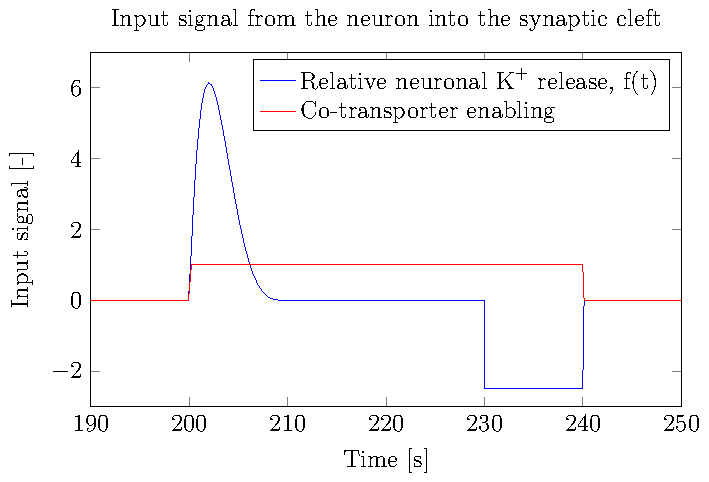
\includegraphics[width = 10cm]{pics/InputSignal.pdf}
	\caption{\textbf{The input signals used in the astrocyte model.} The \gls{K} efflux modelled by a beta distribution and buffered back afterwards (blue). The NKCC1 and KCC1 co-transporters are enabled when the neuronal ion release and spatial buffering is applied, modelled by a block function (red).  }
	\label{fig:InputSignal}
\end{figure}
% 
%
\subsubsection{Scaling}
The flux equations used in the AC model are based on the model of \citet{Ostby2009}. Their intention was to look at the volume changes of the AC and SC, therefore the volumes of both are variables in this model and all fluxes are scaled by a volume-surface ratio ($R_k$ and $R_s$, see Equations \ref{eq:R_k} and \ref{eq:R_tot}, respectively). It is assumed that the sum of the volumes of the AC and SC is a constant ($R_{tot}$). Due to osmotic pressure, the volume changes. We could show that the changes are comparatively small in our model and it would be justifiable to leave out the scaling factors. However, at the moment they are included because the given fluxes of \citet{Ostby2009} are scaled by the volume-surface ratio. It should be considered in future versions to eliminate the scaling factors by multiplying the fluxes with an adequate constant. 




\subsection{SMC and EC Model}
The SMC and EC model is based on the work of \citet{Koenigsberger2006}, see Figure~\ref{fig:SMCECmodel}. This model is extended by adding an inward-rectifier potassium (KIR) channel in the SMC ($ J_{KIR} $, \cite{Filosa2004}) in order to create a connection between the Astrocyte model and the SMC and EC model. \\%A conservation of \gls{K} was added in the SMC and EC model  for the PVS and SMC.\\

The input signal for this model is the \gls{K} concentration in the PVS which is increased by the efflux of astrocytic potassium after neuronal activity. 
\begin{figure}[h!]
  \centering
  \def\svgwidth{450pt} %400pt
  \scriptsize
  \import{pics/}{SMCECmodel3.pdf_tex}
  \caption{\textbf{Illustration of the SMC and EC model.} All modelled fluxes are pictured, note that the indices (k - Astrocyte (AC), s - Synaptic Cleft (SC), p - Perivascular Space (PVS)) are left out for clarity reasons.}
\label{fig:SMCECmodel}
\end{figure}

The raise in \gls{K} in the PVS activates the KIR channel on the SMC, causing them to open extruding more potassium into the PVS. This efflux of \gls{K} hyperpolarizes the SMC membrane and causing the voltage-operated \gls{Ca} channels to close, preventing the influx of \gls{Ca} into the SMC cytosol.\\

The cytosolic \gls{Ca} concentrations in the SMC and EC and that in the sacroplasmatic reticulum (SR) and endoplasmatic reticulum (ER), respectively, are described by a set of differential equations. In- and effluxes  of \gls{K} are given by the following ion channel and pumps: $ J_{KIR} $, $ J_{NaK} $ and $ J_{K} $. \gls{Ca} leaves the SR via the channels: $ J_{CICR} $, $ J_{IP_3} $ and $ J_{SR\_leak} $ and enters it by $ J_{SR\_upt} $. The in- and efflux of \gls{Ca} are modelled with $ J_{extr} $, $ J_{VOCC} $, $ J_{stretch} $ and $ J_{NaCa} $. Note that these fluxes link the cytosol with the extracellular matrix. Here again, a chloride pump is included, $ J_{Cl} $, to return to the resting membrane potential.\\

Physiologically, ECs and SMCs are connected by gap junctions that allow an intercellular exchange of molecules and voltage.  \citet{Koenigsberger2006} include the coupling factors $J_{Ca^{2+}-cpl}^{EC-SMC}$, $V_{cpl}^{EC-SMC}$ and $J_{IP_{3}-cpl}^{EC-SMC}$ for \gls{Ca}, voltage and IP$ _3 $ coupling, respectively. The strength of the coupling can be changed in the code with the variable $ CASE $.\\

Inositol triphosphate (\gls{IP3}) is an important messenger molecule. It's production, in the endothelium, is triggered by agonist binding onto membrane receptors. IP$_3$ mediates the $ J_{IP_3} $ channel, situated between the reticulum and cytosol. 
The production rate of IP3 is a constant over time and can be changed by altering the variable  $ J_{PLC}$ within the mathematical model .\\

Note that the model of \citet{Koenigsberger2006} already includes \gls{Ca}-buffering in the SMC and EC.







%\todo[inline]{What is the expected PLC agonist concentration in the EC?}
%\begin{itemize}
%\item based on \cite{Koenigsberger2006} with a KIR channel added
%\item \todo[inline]{rho as a buffering factor should be added (equation from \cite{Gonzalez1994})}
%\item coupling between EC and SMC included (voltage, Ca, IP3)
%\item \todo[inline]{include stretch activated channels}
%\item the only link between AC model and this model is the potassium efflux through the KIR channel  
%\item \todo[inline]{Potassium conservation of mass equation needs to be included}
%\item Do the NaK pump and the Ki channel lead into the PVS ? (at the moment into nowhere)
%\end{itemize}



%\todo[inline]{Tim's question: Should Ca coupling be included in the membrane potential equation? at the moment there is a voltage coupling, but we want to include also the Ca coupling in the membrane potential equation}

\subsection{Contraction and Mechanical Model}

\subsubsection{Contraction Model}
The contraction and mechanical part of the model is based on the model of \citet{Hai1989}, which describes the formation of cross bridges between the myosin and actin filaments (Figure~\ref{fig:MechModell}). This is coupled with a Kelvin-Voigt model that is used to describe the visco-elastic behaviour of the arterial wall (Figure~\ref{fig:KelvinVoigt}).\\
\begin{figure}[h!]
  \centering
  \def\svgwidth{450pt} %400pt
  \footnotesize
  \import{pics/}{MechanicalModel.pdf_tex}
  \caption{\textbf{Illustration of the contraction model within the smooth muscle cell. }}
\label{fig:MechModell}
\end{figure}

The \gls{Ca} concentration in the SMC is the input signal for the cross bridge model of \citet{Hai1989}. The model uses four possible states for the formation of myosin: free nonphosphorylated cross bridges (M), free phosphorylated cross bridges (Mp), attached phosphorylated cross bridges (AMp) and attached dephosphorylated latch bridges (AM). The dynamics of the fraction of myosin in a particular state is given by four differential equations.\\

The active stress of the SMC is directly proportional to the fraction of attached cross bridges (AM and AMp). Using this model the relation between the cytosolic \gls{Ca} concentration and the active stress of the SMC can be derived.\\

\subsubsection{Mechanical Model}
The fraction of attached myosin cross bridges is the input signal for the visco-elastic mechanical model (Kelvin Voigt, Figure~\ref{fig:KelvinVoigt})  which describes the changes in radius over time. The pressure inside the vessel wall is taken as a constant and the circumferential stress is calculated using the Laplacian law. 


\begin{figure}[h!]
  \centering
  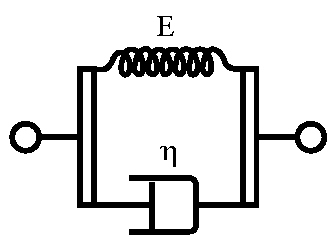
\includegraphics[width = 5 cm]{pics/Kelvin_Voigt_diagram.pdf}
  \caption{\textbf{Schematic overview of a Kelvin Voigt model.}}
  \label{fig:KelvinVoigt}
\end{figure}

The Young's modulus and initial radius of the vessel wall is divided into an active and a passive part and is a function of the attached myosin cross-bridges. The active and passive Young's modulus are based and fitted on experimental data of \citet{Gore} which is shown in Figure~\ref{fig:LinearisationRadius}. 

\begin{figure}[h!]
  \centering
  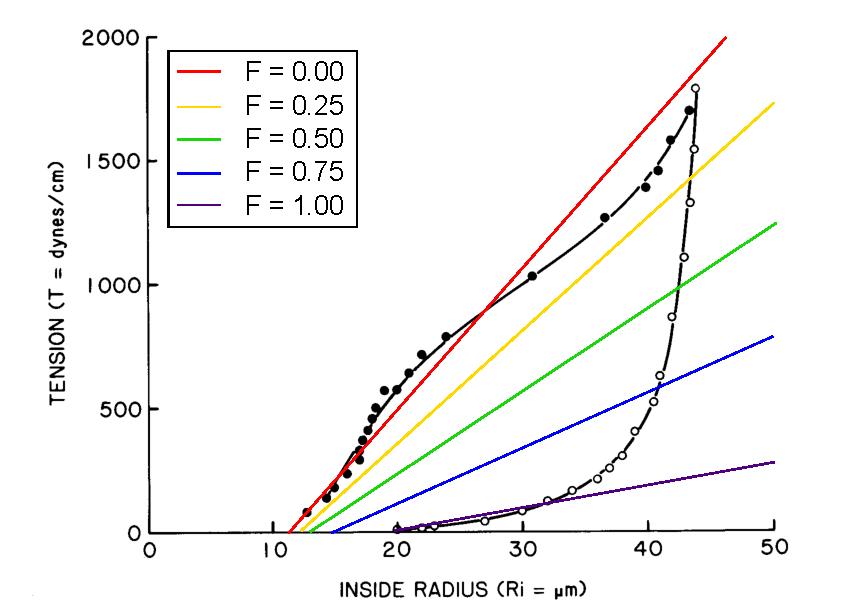
\includegraphics[width = 12 cm]{pics/LinearisationRadius.pdf}
  \caption{\textbf{Linearisation for the Young's modulus and initial radius on the data of \citet{Gore} for different values of F.}}
  \label{fig:LinearisationRadius}
\end{figure}

Figure~\ref{fig:LinearisationRadius} shows that the initial radius ($R_0$) decreases when the fraction of attached myosin cross bridges (F) are increased (the intersection with the x-axis). The figure also shows that the Young's modulus, represented by the slope of the lines in the tension-strain graph, increases when F increases. The linearisations of the Young's modulus can be described by:
\begin{equation} \label{eq:Fbalans4}
T=\frac{\Delta T}{\Delta R}(R-R_0)~,
\end{equation}
where $T$ is the tension of the vessel and $\frac{\Delta T}{\Delta R}$ is the slope of the linearisations in Figure~\ref{fig:LinearisationRadius}. \\

%Gore and Davis et al.\\
\newpage
\subsection{Merging of All Models}

The Astrocyte model and the \gls{SMC} and \gls{EC} model are linked by the SC and the \gls{PVS}. The \gls{K} input signal of the neuron is pumped into the \gls{SC} and taken up afterwards by the AC. The most important ion pumps and channels in this process are the \gls{K} channels in the neuron which releases the \gls{K} input,  the \gls{Na}/\gls{K} pump and \gls{K} channel in the \gls{AC} which pump the released \gls{K} into the AC.
The result of this is an efflux of \gls{K} at the end feet of the astrocyte using the BK-channel. Consequently, the membrane voltage of the astrocyte re-polarizes and the \gls{K} concentration in the PVS increases. This increased \gls{K} concentration activates the KIR channel in the \gls{SMC} and start to pump out more \gls{K} from the \gls{SMC} into the \gls{PVS}. The increased efflux of \gls{K} hyperpolarises the \gls{SMC} membrane voltage and as a result of that the VOCC closes and prevents the influx of \gls{Ca} into the \gls{SMC}.
Summarising, the neuronal input signal leads to a decrease of \gls{Ca} influx by the VOCC channels and therefore a decrease of the intracellular \gls{Ca} concentration. This leads to a decreased fraction of attached myosin bridges in the \citet{Hai1989} model, resulting in vessel dilation in the visco-elastic mechanical model. An overview of the whole model is shown in Figure~\ref{Overview}.

\begin{figure}[h!]
  \centering
  \def\svgwidth{450pt}
  \scriptsize 
  \import{pics/}{All_models_1pt1.pdf_tex}
  \caption{\textbf{All Models.}}
\label{Overview}
\end{figure}






%\begin{itemize}
%%\item What is the real relationship between the Ca concentration and the radius? - more references needed!
%%\item At the moment: Ca input of SMC, cross-bridge model of \citet{HaiMurphy}, Kelvin-Voigt model for elastic response of the arterial wall (assuming Laplace-law), change in radius 
%\end{itemize}

